\chapter{Driving a library from an AI agent}
\label{ch:mcp}

The \lang{dynamic} backend (Chapter~\ref{ch:dynamic}) lets a program ask what
a library contains and call it by name. An AI agent is that kind of program.
The \lang{mcp} target serves your library over the \textbf{Model Context
Protocol}, the open protocol AI assistants use to call external tools. With it,
an agent such as Claude can explore your classes, create objects, set their
fields and call their methods, and read each result before deciding what to do
next:

\begin{quote}
\itshape ``Load the bunny, relax it until its worst triangle is above 0.1, and
tell me how many passes that took.''
\end{quote}

Your headers do not change. The agent reads the documentation rosetta already
carries --- \code{doc} annotations, \code{///} comments, parameter names
(Chapter~\ref{ch:documentation}) --- and stays inside the constraints rosetta
already enforces: \code{range}, \code{readonly}, overload resolution.

\section{What an agent needs, and where it comes from}

An MCP server lists \emph{tools}, each with a name, a description and a JSON
Schema for its arguments; the client calls them and gets JSON back. Every piece
of that already exists in rosetta:

\begin{center}
\small
\begin{tabular}{@{}L{4.6cm}L{8.6cm}@{}}
\toprule
\textbf{The agent needs} & \textbf{Rosetta already has} \\
\midrule
what exists & the registry: classes, enums, free functions \\
what each member means & \code{doc}, harvested comments, parameter names \\
argument types & the \code{TypeDesc} of every field and parameter \\
limits & \code{range} and \code{readonly}, enforced by \code{Object::set} \\
calling by name & \code{resolve()} and the per-member thunks \\
\bottomrule
\end{tabular}
\end{center}

So the \lang{mcp} backend adds no new marshalling layer. It emits the same
metadata tables as \lang{dynamic}, plus a ten-line \code{main()}; everything
protocol-side lives in one reflection-free header,
\code{<rosetta/runtime/mcp.h>}, which knows nothing about your library.

\begin{center}
\begin{tikzpicture}[
  node distance=5mm,
  b/.style={draw,rounded corners=2pt,align=center,font=\scriptsize,inner sep=4pt,text width=25mm,minimum height=11mm},
  user/.style={b,fill=blue!6,draw=rosettablue},
  gen/.style={b,fill=black!4,draw=black!35,dashed},
  fin/.style={b,fill=green!7,draw=green!45!black},
  arr/.style={{Stealth[length=2mm]}-{Stealth[length=2mm]},draw=black!55,font=\scriptsize}
]
\node[fin]  (a) {MCP client\\\scriptsize Claude Code, \ldots};
\node[gen,right=13mm of a] (s) {\texttt{rosetta::mcp::}\\\texttt{Server}\\\scriptsize fixed tools, handles};
\node[gen,right=8mm of s] (r) {\texttt{rosetta::dyn}\\\scriptsize registry, thunks};
\node[user,right=8mm of r] (c) {your classes\\\scriptsize unmodified};
\draw[arr] (a) -- node[above]{JSON} (s);
\draw[arr] (s) -- (r);
\draw[arr] (r) -- (c);
\end{tikzpicture}
\end{center}

\section{A first server}

Add the target next to the others:

\begin{lstlisting}[style=json]
"targets": [
  { "lang": "dynamic", "name": "scene" },
  { "lang": "mcp",     "name": "scene_mcp" }
]
\end{lstlisting}

Generate as usual (Chapter~\ref{ch:rosettagen}); the tree lands in
\code{bindings/mcp/}. Like \lang{dynamic}, it builds with an off-the-shelf
C++20 compiler --- the metadata is data, not splices. The only extra dependency
is nlohmann/json, used if installed and fetched otherwise.

\begin{lstlisting}[style=sh]
cmake -S bindings/mcp -B bindings/mcp/build
cmake --build bindings/mcp/build
claude mcp add scene -- "$PWD/bindings/mcp/build/scene_mcp"
\end{lstlisting}

The last line registers the server with Claude Code; any MCP client takes the
same thing in its JSON configuration. The client launches the executable and
talks to it over stdin/stdout. Start Claude Code, check with \code{/mcp} that
the server is connected, and ask.

\begin{note}
\code{examples/dynamic} has the target already: \code{./run.sh mcp} builds the
server and prints the \code{claude mcp add} line.
\end{note}

\section{From your header to what the agent reads}
\label{sec:mcp-header}

What an agent can do with your library depends on what it can \emph{read} about
it. With the \lang{mcp} target, everything you already wrote for a human ---
doc comments, annotations, parameter names --- is what the agent reads. A small,
complete example shows the path end to end.

\subsection*{The library}

A pendulum, documented the two ways rosetta reads: Doxygen comments, and
annotations. \code{length} and \code{angle} carry \emph{inline} annotations;
\code{damping} and \code{time} are plain C++ and get theirs from a
\emph{side-car} file (Chapter~\ref{ch:annotations}):

\begin{lstlisting}[style=cpp]
#include <rosetta/annotations.h>
#include <cmath>

namespace lab {

    /// A simple pendulum, integrated with a fixed time step.
    class Pendulum {
    public:
        [[= rosetta::doc{"Length of the rod, in metres"}, = rosetta::range{0.1, 10.0}]]
        double length = 1.0;

        [[= rosetta::doc{"Current angle from the vertical, in degrees"},
          = rosetta::range{-90.0, 90.0}]]
        double angle = 30.0;

        double damping = 0.05; // annotated in Pendulum.ann.json
        double time    = 0.0;  // annotated in Pendulum.ann.json

        /**
         * @brief Advance the simulation.
         * @param seconds how long to simulate
         * @param dt      the time step, in seconds
         * @return the angle at the end, in degrees
         */
        double simulate(double seconds, double dt);

        /// Small-angle period, 2 pi sqrt(L/g), in seconds.
        double period() const;
    };
}
\end{lstlisting}

\begin{lstlisting}[style=json]
// Pendulum.ann.json -- the side-car: same vocabulary, outside the header
{
  "damping": { "doc": "Friction coefficient; 0 swings forever", "range": [0, 1] },
  "time":    { "doc": "Simulated time so far, in seconds", "readonly": true }
}
\end{lstlisting}

\begin{lstlisting}[style=json]
"targets": [ { "lang": "mcp", "name": "lab_mcp" } ],
"classes": [ { "name": "lab::Pendulum", "header": "pendulum.h",
               "annotations": "Pendulum.ann.json" } ]
\end{lstlisting}

\subsection*{What the agent reads}

The agent calls \code{describe\_class} on \code{Pendulum} and gets, verbatim
(trimmed to two fields and one method):

\begin{lstlisting}[style=json]
{
  "name": "Pendulum",
  "doc": "A simple pendulum, integrated with a fixed time step.",
  "fields": [
    { "name": "length", "type": "double", "kind": "number",
      "doc": "Length of the rod, in metres", "range": [0.1, 10.0] },
    { "name": "time", "type": "double", "kind": "number",
      "doc": "Simulated time so far, in seconds", "readonly": true }
  ],
  "methods": [
    { "name": "simulate",
      "signature": "simulate(double seconds, double dt) -> double",
      "doc": "Advance the simulation.\n\nArgs:\n    seconds: how long to simulate\n    dt: the time step, in seconds\n\nReturns:\n    the angle at the end, in degrees",
      "params": [ { "name": "seconds", "type": "double", "kind": "number" },
                  { "name": "dt",      "type": "double", "kind": "number" } ] }
  ]
}
\end{lstlisting}

Every line of it traces back to something in the header or the side-car:

\begin{center}
\small
\begin{tabular}{@{}L{4.3cm}L{4.0cm}L{4.9cm}@{}}
\toprule
\textbf{You wrote} & \textbf{The agent reads} & \textbf{So it can} \\
\midrule
\code{///} above the class & the class \code{doc} in \code{list\_classes}
  and \code{describe\_class} & pick the right class for the request \\
\addlinespace
\code{doc\{\ldots\}}, inline or side-car & a field's \code{doc} & know what
  \code{damping} means, and its unit \\
\addlinespace
\code{range\{lo, hi\}}, inline or side-car & \code{"range": [lo, hi]} &
  choose valid values --- and is \emph{stopped} if it does not \\
\addlinespace
\code{readonly}, inline or side-car & \code{"readonly": true} & treat the field
  as an output, never set it \\
\addlinespace
\code{@brief}, \code{@param}, \code{@return} & the method \code{doc}, with
  \code{Args:} and \code{Returns:} sections & call it with the right arguments,
  and interpret the result \\
\addlinespace
the parameter names & \code{params[].name}, the signature & pass arguments by
  name: \code{\{"seconds": 1.4, "dt": 0.001\}} \\
\addlinespace
the C++ types & \code{type} and \code{kind} & send a number, a string, a
  handle, an enumerator name \\
\addlinespace
\code{combobox\{\ldots\}} & \code{"choices": [\ldots]} & offer one of them
  (listed, not enforced) \\
\bottomrule
\end{tabular}
\end{center}

\subsection*{And what happens when it gets something wrong}

The same annotations are \emph{enforced} at call time, by the core --- not by
the agent's good will. From a session against this server:

\begin{lstlisting}[style=plain]
set_fields {"object": "p", "values": {"length": 25, "time": 3}}
  -> error: updated []; rejected:
       length = 25 is outside [0.1, 10]
       Pendulum::time is read-only

set_fields {"object": "p", "values": {"length": 2.0, "damping": 0}}
  -> {"updated": ["damping", "length"]}

call_method {"target": "p", "method": "period"}
  -> {"result": 2.837006706885772}

call_method {"target": "p", "method": "simulate",
             "args": {"seconds": 1.418, "dt": 0.001}}
  -> {"result": -29.960569829913847}
\end{lstlisting}

The \code{range} that the agent read in \code{describe\_class} is the one that
rejects \code{length = 25}; the side-car's \code{readonly} is the one that
protects \code{time}. Having read the documentation of \code{period()}, the
agent can sanity-check the model: simulated for half a period with no damping,
the pendulum ends at $-30^\circ$, the mirror of its starting angle.

\begin{note}
\textbf{Inline or side-car?} They produce the same metadata and can be mixed,
as above. The difference is who has to compile your header. The \lang{mcp}
server --- like \lang{dynamic} --- includes it, and inline annotations make it
C++26 source, so a header annotated inline needs the C++26 toolchain to build
the server too. With side-car annotations the header stays plain C++ and the
server builds with an off-the-shelf compiler. That is why
\code{examples/dynamic} keeps every annotation in \code{*.ann.json} files ---
and it is the natural choice for a third-party library you do not want to
touch.
\end{note}

\begin{warn}
Default arguments do not reach the dynamic tables: the agent must pass every
parameter (\code{simulate(1)} is rejected as ``takes 2 argument(s), 1 given'').
Document the value you would have defaulted, so the agent knows what to send.
\end{warn}

\section{What a conversation looks like}
\label{sec:mcp-chats}

The point of all this is not that an agent can call \code{set\_fields}. It is
that you can ask a \emph{question about your domain} and the agent works out
which calls answer it. The five conversations below were run against the
pendulum server of Section~\ref{sec:mcp-header}, with Claude Opus 5.5 through
Claude Code, connected to that server and nothing else (no shell, no files).
Replies are abridged, not rewritten; the agent's scripts are excerpted, with
some comments added. Every session started with the same two calls ---
\code{list\_classes}, then \code{describe\_class} --- which is how the agent
learned everything it knew about the library.

\subsection*{1. ``What can this library do?''}

\begin{quote}
\small\itshape
What can this library do? Give me a one-paragraph tour.
\end{quote}

\begin{quote}
\small
This library has one class, \code{lab::Pendulum}, which simulates a simple
pendulum using a fixed time step. You create one with no arguments and set three
fields: \code{length} (0.1--10\,m), \code{angle} (the starting angle from
vertical, $-90^\circ$ to $90^\circ$) and \code{damping} (a friction coefficient
from 0 to 1, where 0 means it swings forever). A read-only \code{time} field
counts the simulated seconds so far. \code{simulate(seconds, dt)} runs the
simulation forward and returns the final angle in degrees; \code{period()}
returns the small-angle period, $2\pi\sqrt{L/g}$. [\ldots]
\end{quote}

Every fact in that paragraph is a \code{doc}, a \code{range}, a
\code{readonly}, a parameter name or a \code{@return} from the header and the
side-car. Nothing was guessed.

\subsection*{2. Asking for something the library refuses}

\begin{quote}
\small\itshape
Make a pendulum with a 15 metre rod and release it from 120 degrees.
\end{quote}

\begin{quote}
\small
I couldn't build that pendulum: both values are outside what the library
allows. \code{Pendulum.length} only accepts 0.1--10\,m [\ldots]
\code{Pendulum.angle} only accepts $-90^\circ$ to $90^\circ$ [\ldots] I haven't
created any object. Which would you like? (1) a 10\,m rod released from
$90^\circ$; (2) keep the 15\,m rod's swing shape at a length the library
accepts --- swing timing scales with $\sqrt{L}$, so multiply the times by
$\sqrt{1.5} \approx 1.22$; (3) different values within the limits.
\end{quote}

The agent never called \code{set\_fields}: it read the two \code{range}
annotations in \code{describe\_class} and declined \emph{before} touching the
C++ side --- then offered a physically sound workaround. Had it tried anyway,
the core would have rejected the values (Section~\ref{sec:mcp-header}).

\subsection*{3. An inverse problem}

\begin{quote}
\small\itshape
I want a pendulum that ticks once per second, i.e.\ a period of exactly
2 seconds. What rod length do I need? Set it on a pendulum and verify it by
simulation.
\end{quote}

The agent answered with \emph{one} \code{run\_script} call. It recovered $g$
from \code{period()} itself rather than assuming it, set the length, then timed
the swing from its zero crossings:

\begin{lstlisting}[style=plain]
local p = new("Pendulum")
p.length = 1
local g = 4*math.pi^2 / p:period()^2   -- the library's own g
p.length = g / math.pi^2               -- T = 2 s
p.damping, p.angle = 0, 2              -- small swing, no friction
-- step with dt = 1e-4, record the upward zero crossings,
-- average the period over the crossings found in 20 s
...
-> {"L": 0.9939608115313356, "period_formula": 2,
    "T_sim": 2.0001523111193213, "n_periods": 9}
\end{lstlisting}

\begin{quote}
\small
You need a rod length of $L = gT^2/4\pi^2 = g/\pi^2 \approx 0.99396$\,m. I set
\code{length} to that value: \code{period()} returns 2.000000\,s, and a
simulation timed over 9 full swings gives 2.00015\,s. The extra 0.00015\,s is a
real effect of swinging at a non-zero angle, not a simulation error: at
$2^\circ$ the expected period is $T_0(1 + \theta^2/16) \approx 2.00015$\,s.
\end{quote}

\subsection*{4. A numerical search}

\begin{quote}
\small\itshape
Starting from 30 degrees, what damping makes the swing amplitude drop to half
after 20 seconds of simulation? Find it numerically.
\end{quote}

Again one script: a function measuring the amplitude over the last period before
$t = 20$\,s, then 40 steps of bisection on \code{damping}, run twice with
different time steps to check convergence (3.6\,s inside the server):

\begin{lstlisting}[style=plain]
local function amp(c, dt) ... end       -- largest |angle| in the last period
local lo, hi = 0, 1
for i = 1, 40 do
  local mid = (lo + hi) / 2
  if amp(mid, 0.001) > 15 then lo = mid else hi = mid end
end
-> c(dt=1e-3) = 0.075475,  c(dt=2e-4) = 0.075476
\end{lstlisting}

\begin{quote}
\small
The damping that halves the swing amplitude after 20\,s is
$c \approx 0.0755$. With no damping the amplitude stays at $30.00^\circ$, so the
integrator isn't adding or losing energy on its own, and the result doesn't
depend on the time step. This is a bit higher than $2\ln 2/20 \approx 0.0693$,
the textbook value for linear damping. \textbf{The library doesn't document its
damping law}, so this difference may come from how it applies friction or from
the swing being large.
\end{quote}

That last sentence is worth noticing: the agent is exactly as precise as your
documentation. The header says what \code{damping} is for, not how it enters
the equation of motion, and the agent says so instead of pretending. One more
line in the \code{doc} --- ``$\ddot\theta = -(g/L)\sin\theta - c\,\dot\theta$''
--- and it could have reasoned about the difference too.

\subsection*{5. Testing the model's own assumptions}

\begin{quote}
\small\itshape
Is the small-angle period formula still accurate if I release the pendulum
from 80 degrees? Measure the real period by simulation and compare.
\end{quote}

The agent timed the period at $5^\circ$ and $80^\circ$, each at two time steps,
in one script, and compared it with \code{period()}:

\begin{center}
\small
\begin{tabular}{@{}lccc@{}}
\toprule
\textbf{Release angle} & \textbf{Simulated period} &
  \textbf{\code{period()}, $2\pi\sqrt{L/g}$} & \textbf{Error} \\
\midrule
$5^\circ$  & 2.0070\,s & 2.0061\,s & 0.05\,\% \\
$80^\circ$ & 2.2819\,s & 2.0061\,s & \textbf{13.75\,\%} \\
\bottomrule
\end{tabular}
\end{center}

\begin{quote}
\small
No, not at $80^\circ$: the small-angle formula is about 14\,\% too short. The
real period is 1.1375 times the formula's value, which matches the exact
large-amplitude result $T = T_0\,(2/\pi)\,K(\sin(\theta_0/2))$. The formula
assumes $\sin\theta \approx \theta$; at large angles the restoring force is
weaker, so the pendulum swings more slowly. Rule of thumb: the error is about
$\theta_0^2/16$, which stays under 1\,\% up to about $23^\circ$.
\end{quote}

The library provided the two primitives, \code{simulate} and \code{period};
the agent combined them into an experiment, checked convergence, and connected
the numbers to the physics --- including where the library's own
\code{period()} stops being valid.

\subsection*{What made these possible}

\begin{itemize}
  \item \textbf{The documentation was the interface.} Units, ranges, what each
    parameter means, what a method returns: the agent used all of it, and named
    the one thing that was missing.
  \item \textbf{Scripts turned questions into one call.} Sessions 3--5 each took
    four turns in total, the work being a single \code{run\_script}; the same
    experiments as individual tool calls would have needed hundreds of round
    trips.
  \item \textbf{The C++ did the computing.} The agent wrote the experiment and
    read the result; every number came from your \code{simulate()}.
\end{itemize}

To reproduce them, point Claude Code at the server and ask:

\begin{lstlisting}[style=sh]
claude mcp add lab -- "$PWD/lab_mcp"
claude
\end{lstlisting}

\section{The tools}

The agent always sees the same small set, whatever the library:

\begin{center}
\small
\begin{tabular}{@{}lL{9.6cm}@{}}
\toprule
\textbf{Tool} & \textbf{Does} \\
\midrule
\code{list\_classes} & classes (with their static factories), enums, free
  functions --- the agent starts here \\
\code{describe\_class} & constructors; fields with type, doc, range, choices,
  enum values, read-only; methods with signature and doc. Inherited members
  included \\
\code{create\_object} & best-matching constructor; returns a handle and the new
  object's fields \\
\code{call\_method} & a method on a handle, or a static method when
  \code{target} is a class name; \code{store\_as} names a returned object \\
\code{inspect\_object} & every readable field at once \\
\code{set\_fields} & several assignments in one call, each validated \\
\code{list\_objects}, \code{release\_object} & the handle table \\
\code{call\_function} & free functions (listed only when some are bound) \\
\code{run\_script}, \code{run\_python} & a script run next to the objects ---
  Section~\ref{sec:mcp-scripts} \\
\bottomrule
\end{tabular}
\end{center}

\subsection*{Why not one tool per method}

Generating \code{Mesh\_subdivide}, \code{Relaxer\_run}, \ldots{} would look more
direct, and scales badly: agents pick tools less reliably as the list grows,
every schema costs context on every turn, and a 500-class library would produce
thousands. With a fixed set, discovery is \code{describe\_class}, paid only for
the classes the agent actually touches --- and the tool list never changes when
the library grows.

\subsection*{Handles}

Tool calls are stateless; the server process is not. Live objects sit in a
handle table, under \code{<Class>\#<n>} or a name the agent chooses. A handle
goes back in as \code{\{"\$ref": "bunny"\}}, or as the bare string
\code{"bunny"} wherever the parameter's type is known to be a class:

\begin{lstlisting}[style=json]
call_method   {"target": "Mesh", "method": "bunny", "store_as": "bunny"}
  -> {"result": {"$ref": "bunny", "class": "scene::Mesh"}}
call_method   {"target": "Relaxer", "method": "minQuality", "args": ["bunny"]}
  -> {"result": 0.014254101544304952}
\end{lstlisting}

A \code{T\&} return comes back as a handle that \emph{pins} its parent, exactly
as in Chapter~\ref{ch:dynamic}: release the mesh, and a handle to its
\code{origin} stays valid. Each handle reports whether it is \code{owned},
\code{pinned} or \code{borrowed}.

\subsection*{Arguments}

JSON has no enums, no classes and no int/double distinction, so arguments are
converted against the parameter type wherever it can be known. Arguments may
be positional (\code{"args": [1, 2]}) or by parameter name
(\code{"args": \{"m": "bunny"\}}) --- the names are the ones reflected from your
declarations. Enum values are passed and returned by enumerator name.

\subsection*{Bulk data is summarised}

A vector longer than 64 elements does not come back whole. An agent needs to
know a mesh has 35\,947 vertices and roughly where they are, not to read 107\,841
doubles into its context:

\begin{lstlisting}[style=json]
call_method {"target": "bunny", "method": "positions"}
  -> {"result": {"$summary": true, "length": 107841,
                 "head": [-0.134, 0.114, 0.037, ...],
                 "min": -0.5002, "max": 0.5002, "mean": -0.0308}}
\end{lstlisting}

A script, on the other hand, receives vectors whole
(Section~\ref{sec:mcp-scripts}).

\section{Constraints the agent cannot bypass}

Everything the core enforces stays enforced, and a rejection comes back as a
\emph{tool error} with the core's own message --- which is what lets the agent
correct itself on the next call. From a real session on the \code{scene}
library:

\begin{lstlisting}[style=plain]
set_fields {"object": "bunny",
            "values": {"opacity": 7, "shading": "Wireframe", "id": "x"}}
  -> error: updated ["shading"]; rejected:
       Mesh::id is read-only
       opacity = 7 is outside [0, 1]

call_method {"target": "bunny", "method": "at", "args": ["nope"]}
  -> error: Mesh::at(std::string) matched no overload of 2:
       at(int) -- argument 1 ("nope") is not a int
       at(int, int) -- takes 2 argument(s), 1 given

call_method {"target": "bunny", "method": "onProgress", "args": [1]}
  -> error: ... onProgress(std::function<void(double)>) -- not callable:
       callback: a std::function parameter needs a foreign-callable adapter
\end{lstlisting}

The valid assignment in the first call (\code{shading}) still lands; only the
two refused ones are reported.

\begin{warn}
There is no authorisation model beyond your annotations: anything bound can be
called. Bind only what an agent should be able to reach, and use
\code{readonly} and \code{range} for what it may read but not freely change.
\end{warn}

\section{Scripts: one call instead of dozens}
\label{sec:mcp-scripts}

Every tool call is a round trip through the model. ``Relax until the worst
triangle passes 0.1'' as individual calls --- run, measure, decide, repeat ---
takes dozens of them, each one re-reading the conversation. As a script it is
one:

\begin{lstlisting}[style=plain]
-- run_script: Lua, next to the live objects
local m = obj("bunny")
local r = new("Relaxer")
r.iterations, r.step = 1, 0.7
local passes = 0
while classes.Relaxer.minQuality(m) <= 0.1 do
  r:run(m)
  passes = passes + r.lastPasses
end
return {passes = passes, worst = classes.Relaxer.minQuality(m)}
\end{lstlisting}

On the Stanford bunny this returns \code{\{passes = 1, worst = 0.1534\}}: the
worst triangle went from 0.0143 to 0.1534 in a single tool call.

Both scripting tools see the same small API, which their tool descriptions spell
out for the agent:

\begin{center}
\small
\begin{tabular}{@{}L{3.2cm}L{4.6cm}L{5.4cm}@{}}
\toprule
 & \textbf{Lua} (\code{run\_script}) & \textbf{Python} (\code{run\_python}) \\
\midrule
fetch a handle & \code{obj("bunny")} & \code{obj("bunny")} \\
construct & \code{new("Relaxer")}, \code{classes.Relaxer()} & same \\
field & \code{o.step = 0.7} & same \\
method & \code{o:run(m)} & \code{o.run(m)}, keyword arguments too \\
static method & \code{classes.Relaxer.\bk minQuality(m)} & same \\
publish a handle & \code{keep("name", o)} & same \\
result & the \code{return} value & the last expression, as in a notebook \\
\bottomrule
\end{tabular}
\end{center}

They go through the same core as the JSON tools --- a range violation is a Lua
error (catchable with \code{pcall}) or a Python \code{RuntimeError} --- and
share the handle table, so an object made in a script is a handle for the next
tool call. Unlike the JSON tools, scripts get vectors \emph{whole}: running next
to the data is the point. Only what a script returns is summarised, and
\code{print()} is captured.

\begin{lstlisting}[style=py]
# run_python: the environment comes with it
import numpy as np
a = np.array(obj("bunny").positions()).reshape(-1, 3)
{"bbox_min": a.min(0), "bbox_max": a.max(0)}
\end{lstlisting}

\subsection*{Lua is sandboxed; Python is not}

\begin{center}
\small
\begin{tabular}{@{}L{3.0cm}L{5.0cm}L{5.2cm}@{}}
\toprule
 & \code{run\_script} (Lua) & \code{run\_python} \\
\midrule
built when & Lua 5.3+ is found (default) & \code{-DROSETTA\_MCP\_PYTHON=ON} \\
reaches & the bound library only: no \code{io}, \code{os}, \code{require},
  \code{load} & everything the server process can \\
limits & wall clock (default 30\,s), Lua heap (512\,MB) & wall clock; raises
  \code{TimeoutError} \\
brings & nothing else & numpy and the whole environment \\
\bottomrule
\end{tabular}
\end{center}

\begin{warn}
CPython cannot be meaningfully sandboxed from inside. With \code{run\_python}
enabled, an agent's script runs with the server's own permissions --- it can
read your files and start processes. That is why it is off by default, and why
its tool description says so. Enable it only for an agent you would let run
Python on that machine anyway.
\end{warn}

Neither language can interrupt a long call into C++: that is your library's
own code, and it finishes.

\section{Inside a running application}

The stdio server is a process the client launches, so it owns its own objects:
nothing it does shows up in an application that is already open. The other way
round is often what you want --- the agent working on the objects the
application is \emph{showing}.

\code{<rosetta/runtime/mcp\_qt\_http.h>} does that for a Qt application. It
serves the same \code{Server} over HTTP on \code{127.0.0.1}, on the GUI thread,
so a tool call runs between two frames and needs no locking against the code
that draws. The Qt viewer of \code{examples/dynamic} starts it at launch:

\begin{lstlisting}[style=sh]
./run.sh viewer
#   console: MCP server for this scene: http://127.0.0.1:8770/mcp
claude mcp add --transport http scene-viewer http://127.0.0.1:8770/mcp
\end{lstlisting}

Ask Claude Code to ``subdivide the sphere and make it glossy'', and the sphere
goes from 768 to 3\,072 triangles in the 3-D view while you watch; the viewer's
console logs each outside call (\code{[mcp] call\_method \ldots}).

\begin{note}
The host binds to the loopback interface only and refuses requests whose
\code{Origin} is not localhost, so a web page cannot drive it. There is no
authentication: any local process can connect, as any local process could run
the stdio binary. \code{ROSETTA\_MCP\_PORT} changes the port; \code{0} turns the
host off.
\end{note}

\subsection*{The viewer's own Claude tab}

The viewer also has a \textbf{Claude} tab next to its console, with two
backends:

\begin{itemize}
  \item \textbf{Claude Code (your login)}, the default when \code{claude} is
    installed. Like the VS Code extension, the tab runs the Claude Code CLI for
    each message --- with \code{ANTHROPIC\_API\_KEY} removed, so your Claude Code
    subscription is used --- connected to the viewer's own MCP server and to
    nothing else: no shell, no file access.
  \item \textbf{Anthropic API}, which calls the Messages API directly and needs
    an \code{ANTHROPIC\_API\_KEY} with credits.
\end{itemize}

Either way the transcript shows Claude's replies, each tool call (scripts as
code) and its result, and the scene updates after every call.
Figure~\ref{fig:mcp-viewer} shows it.

% Same guard as the title-page logo: a copy of docs/book without the
% figures/ directory still builds, it just loses the screenshot.
\begin{figure}[ht]
\centering
\IfFileExists{figures/mcp.png}{%
  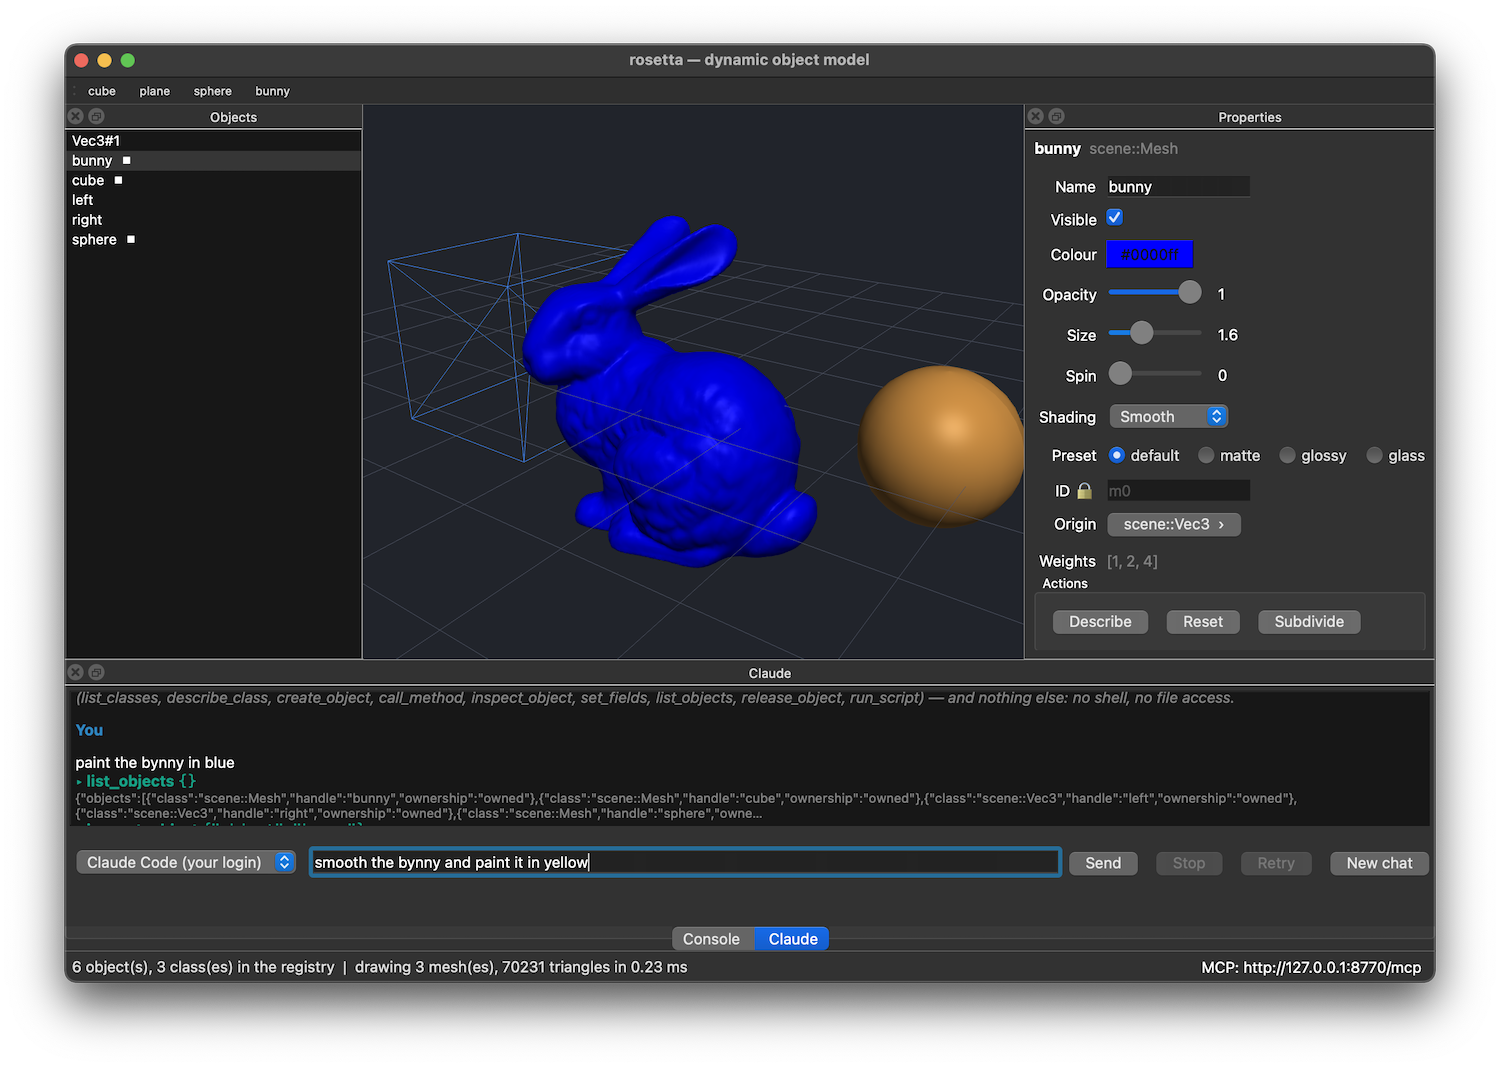
\includegraphics[width=\textwidth]{figures/mcp.png}%
}{\fbox{\small figures/mcp.png is missing}}
\caption{The Claude tab of the \code{examples/dynamic} viewer, on the Claude
  Code backend. Asked to ``paint the bunny in blue'', Claude listed the objects
  (\code{list\_objects}) and set the bunny's \code{colour}; the 3-D view and the
  property panel show the result, and the next request is being typed. The
  status bar shows the viewer's own MCP endpoint.}
\label{fig:mcp-viewer}
\end{figure}

\section{Embedding it in your own application}

All of the above is a few lines over the runtime headers. This is the shape of
the viewer's own wiring:

\begin{lstlisting}[style=cpp]
#include <rosetta/runtime/mcp.h>
#include <rosetta/runtime/mcp_lua.h>      // run_script
#include <rosetta/runtime/mcp_qt_http.h>  // QtHttpHost

scene::register_all();                    // your generated metadata

rosetta::mcp::Server server({.name = "my-app"});
rosetta::mcp::enable_lua(server);         // optional

// Publish objects the application already owns, under the names it uses.
const auto *meshClass = rosetta::dyn::registry().find_class("scene::Mesh");
server.put("bunny", rosetta::dyn::Object::borrow(*meshClass, &myMesh));

rosetta::mcp::QtHttpHost host(server);
host.set_handler([&](const rosetta::mcp::json &msg) {
    auto reply = server.handle(msg);      // one JSON-RPC message
    if (msg.value("method", "") == "tools/call")
        view->update();                   // the agent changed something
    return reply;
});
host.listen(8770);
\end{lstlisting}

The other entry points, for a non-Qt host or a test:

\begin{itemize}
  \item \code{server.serve\_stdio()} --- the generated \code{main()}; diverts
    \code{std::cout} to stderr so a chatty library cannot corrupt the protocol.
  \item \code{server.handle(json)} --- one message in, one reply out, no I/O:
    the whole protocol is testable without a pipe.
  \item \code{server.add\_tool(definition, fn)} --- your own tools next to the
    generic ones. \code{run\_script} and \code{run\_python} are added exactly
    this way.
\end{itemize}

\section{Limits}

\begin{itemize}
  \item \textbf{The agent orchestrates; it does not compute.} Loops belong in
    a script, heavy numerical work in your C++ methods.
  \item \textbf{No callbacks.} \code{std::function} parameters are described
    but not callable, as in every dynamic consumer.
  \item \textbf{No persistence.} Handles live as long as the server process
    --- the client session for stdio, the application for the Qt host.
  \item \textbf{Positional enum names across disagreeing overloads} stay
    strings; pass the integer value or use named arguments.
\end{itemize}

The design note \code{docs/MCP.md} has the reasoning behind each decision and
the list of next steps.
